\section{Using DISCO with Other Systems}
\label{sec:other_systems}

\subsection{Getting DISCO to read your files}
\begin{figure}
	\centering
	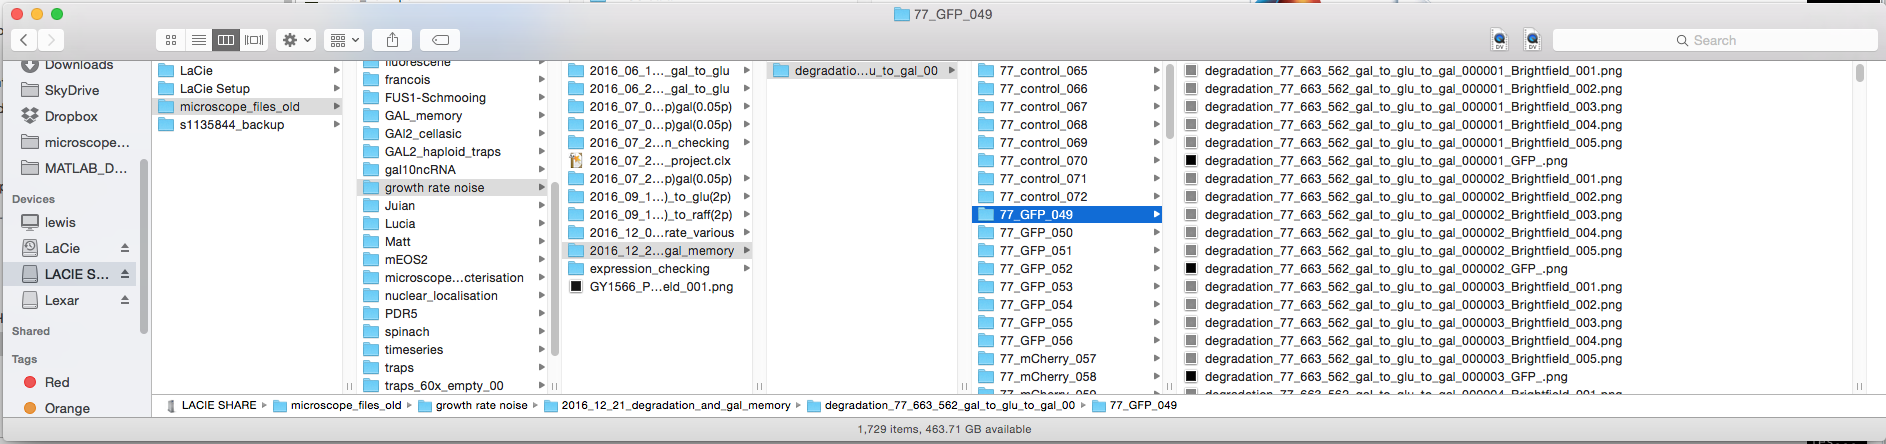
\includegraphics[width=1\linewidth]{documentation_images/other_systems-swain_file_structure}
	\caption[swain lab image file system]{An example of how images are stored in the swain lab image file system. The example shows and experiment called \texttt{degradation\_77\_663\_562\_gal\_to\_glu\_to\_gal\_00} in which Brightfield was imaged with 5 z slices and GFP was imaged with only 1. }
	\label{fig:other_systems-swain_file_structure}
\end{figure}
In order to be able to process the images in anyway, DISCO must of course be able to load your files and therefore know where they are.\\
The DISCO software was designed to be used with files generated by the swain lab microscope control software, which stores files in the form:
\begin{verbatim}
[experiment name]_[6 character timepoint]_[channel name]_[3 character z-slice].png
\end{verbatim}
with each position being stored in a separate folder. An example is shown in figure \ref{fig:other_systems-swain_file_structure}. This is (I believe) also the convention followed by MicroManager. If you're files are arranged in a different structure an you wish to make the software work, there are two options open to you.

\subsubsection{Easy Option: Export Images using ImageJ}
\begin{figure}
\centering
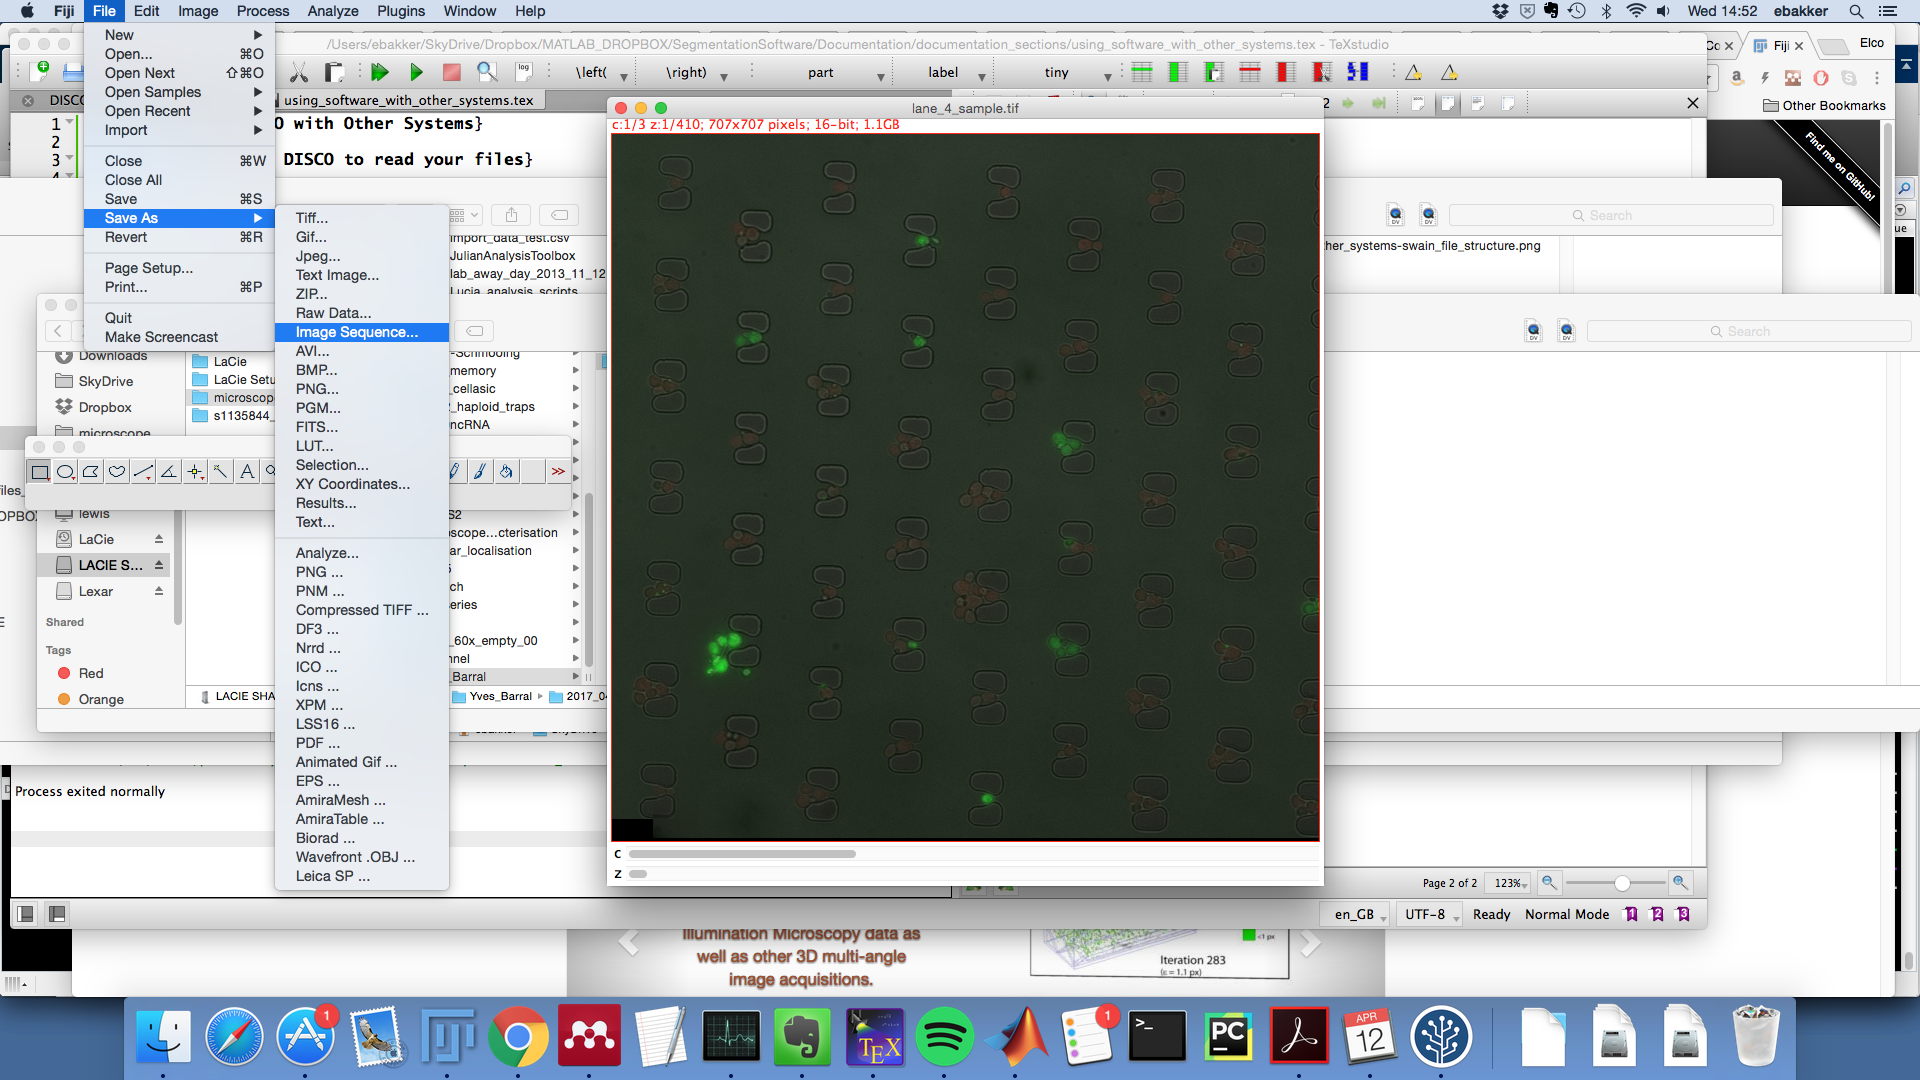
\includegraphics[width=1\linewidth]{documentation_images/other_systems-exporting_from_FIJI}
\caption[Exporting images for processing from FIJI]{Exporting images for processing from FIJI. Shown is the `save' options that should be selected for exporting an image stack for processing from FIJI. Selecting this option will open a dialogue box in which `format' should be set to PNG and `digits' should be set to 6.}
\label{fig:other_systems-exporting_from_FIJI}
\end{figure}


The easiest option is to use ImageJ or \href{https://fiji.sc/}{FIJI} to save your images in this format. These programs can handle most image formats and file structures.\\
First load in an images stack in a way you are happy with. Then save the image stack as an image sequence, choosing a format of PNG and Digits as 6. This will store the image sequence in format appropriate for the software, with channel names given as \texttt{c000001,c000002,c000003 ...}\\
If multiple image stacks are to be processed they can be saved to separate folders in the same parent folder (in imitation of the Swain Lab file structure), allowing the software to be conveniently run on all of them.

\subsubsection{Developer Option: Modify \texttt{timelapseTraps} Constructor and \texttt{timelapseTraps.addChannelsTimelapse} method.}